\section{Analysis and Future Directions}
In this section, we first present a statistical analysis of the papers 
covered in this survey. Then, some future directions are proposed inspired by
our observations.
\begin{figure}[htbp]
	\centering
	\begin{minipage}[t]{0.45\linewidth}
		\centering
		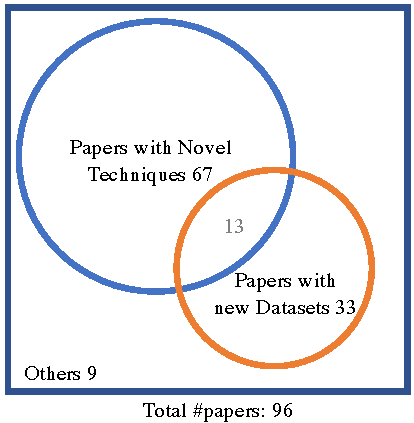
\includegraphics[scale=0.6]{fig/distribution1.pdf}
		\caption{Statistics of abstractive dialogue \\summarization papers.}
		\label{fig:papers}
	\end{minipage}
	\begin{minipage}[t]{0.45\linewidth}
		\centering
		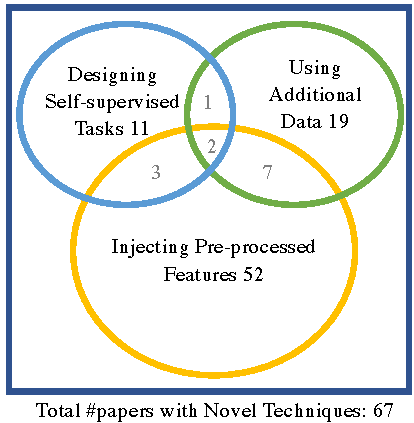
\includegraphics[scale=0.6]{fig/distribution2.pdf}
		\caption{Statistics of papers with technical contributions.}
		\label{fig:technical}
	\end{minipage}
\end{figure}
\subsection{Paper Analysis}\label{sec:observations}
The total number of papers on abstractive dialogue summarization investigated 
in this survey is $96$. 
As shown in \figref{fig:papers}, $33$ of them propose new datasets and 
$67$ make novel technical contributions. The other $9$ papers are either 
a survey, a demo, or other strongly related papers. 
The overall ratio between technical papers and dataset papers 
(\textit{tech-data ratio}) is around $2.03:1$. Compared with the number of 
papers under different application scenarios in \figref{fig:tech-data}, 
we found that scenarios of daily chat and official issues receive more 
attentions, which is evident from the larger number of papers and 
greater tech-data ratios of more than $3$.
However, the other scenarios are less explored, with much lower 
tech-data ratios ranging from $1.0$ to $1.75$.
There is no significant difference in the number of datasets between
well-researched domains and the others. However, the release time and availability of different datasets vary.
AMI and ICSI are well-known meeting summarization datasets released in the early stage of the $20$th century, while most other datasets have been proposed in recent years.
Datasets for daily chat are all publicly available, while datasets for medical care and laws are not accessible to the majority of researchers. It's a good sign that high-quality corpora, such as AMI and SAMSum, lead to a prosperous of techniques for dialogue summarization, but also raise a worry about the generalization ability of current techniques because of their over-reliance on specific datasets which may lead to over-fitting.

%\KZ{Not sure what you mean here: This phenomenon is largely caused by 
%the availability and the release time of corresponding datasets.
%For example, AMI and ICSI are well-known meeting summarization datasets released at the early of the $20$th century while other datasets are most proposed in recent years.
%Datasets for daily chats are all free online, while datasets for medical care are not accessible to general researches.}

%\JQ{Differences between pre-processed features and non-labored techniques is unclear}
The distribution of technical papers in each of the three research directions 
is shown in \figref{fig:technical}.
While $11$ and $19$ papers focus on designing self-supervised tasks and 
using additional data, respectively, 
more than $77\%$ of the entire body of works targets the injection of 
pre-processed features. The trends of paper account for different techniques 
across scenarios that are similar to each other according to the statistics 
in \figref{fig:tech-scenario}. IPF, DST, and UAD are short for injecting pre-processed features, designing self-supervised tasks, and using additional data, respectively.
The number of papers using features under different categories is 
shown in Figure~\ref{fig:feature-scenario}. 
%Intuitively, all features mentioned in Section \ref{sec:feature} are suitable for both ODS and TDS, except roles and domain knowledge which are only for TDS. However, \citet{fabbri2021convosumm} mentioned that their proposed argument graph doesn't benefit shorter and more linear dialogues such as their newly released e-mail data. This reminds us rethinking about whether different features are suitable for all kinds of dialogues.
And based on these $52$ paper, we go for a deep insight into 
correlations between features and applications scenarios by categorizing 
papers according to features and their tested scenarios in 
Table~\ref{tab:correlation}. 

\begin{figure}[ht]
	\centering
	\subfigure[]{
	\begin{minipage}[t]{0.3\linewidth}
	\centering
	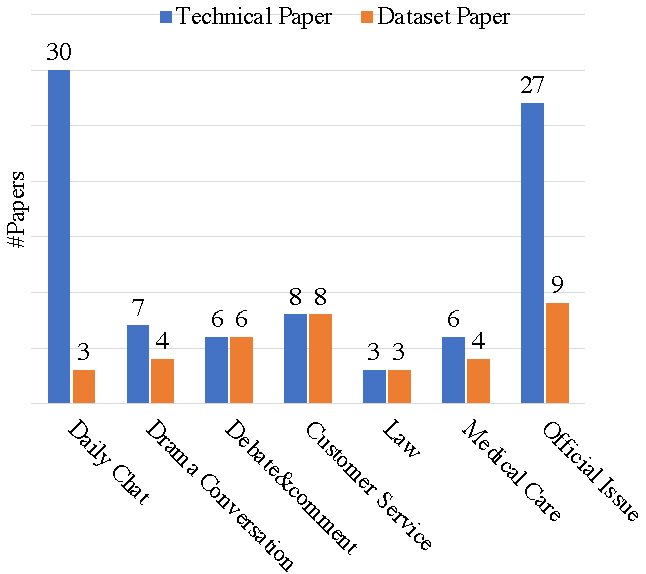
\includegraphics[scale=0.4]{fig/tech-data.pdf}
	%\caption{The number of technical papers and \\dataset papers under different scenarios.}
	\label{fig:tech-data}
	\end{minipage}}
	\subfigure[]{
	\begin{minipage}[t]{0.3\linewidth}
	\centering
	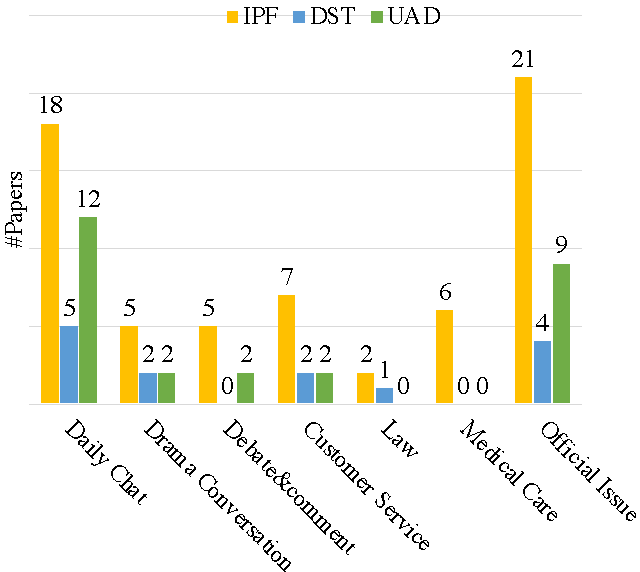
\includegraphics[scale=0.4]{fig/tech-scenario.pdf}
	%\caption{The number of technical papers dividing by directions under different scenarios. IPF, DST and UAD are short for the three directions.}
	\label{fig:tech-scenario}
	\end{minipage}}
	\subfigure[]{
	\begin{minipage}[t]{0.3\linewidth}
	\centering
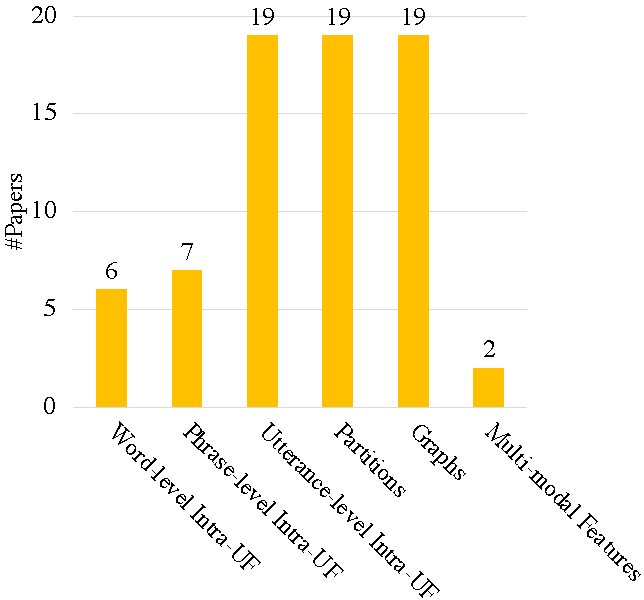
\includegraphics[scale=0.38]{fig/feature-scenario.pdf}
%\caption{The number of technical papers under different features. Intra-UF is short for intra-utterance features. }
\label{fig:feature-scenario}
\end{minipage}}
\caption{(a) The number of technical papers and dataset papers under different scenarios. (b) The number of technical papers dividing by directions under different scenarios. IPF, DST and UAD are short for the three directions. (c) The number of technical papers under different features. Intra-UF is intra-utterance features.}
\end{figure}




%\begin{figure}[htbp]
%	\centering
%	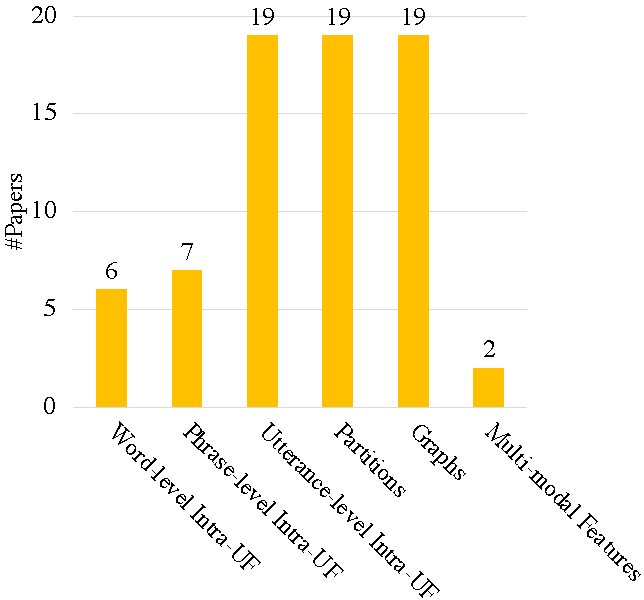
\includegraphics[scale=0.5]{fig/feature-scenario.pdf}
%	\caption{The number of technical papers under different features. Intra-UF is short for intra-utterance features. }
%	\label{fig:feature-scenario}
%\end{figure}

\begin{table}
	\centering
	\begin{tabular}{|l|ccc|cc|c|}
		\toprule[1pt]
		\multicolumn{1}{|c|}{\multirow{2}{*}{\diagbox{Scenarios}{Features}}} & \multicolumn{3}{c|}{\textbf{Intra-Utterance Features}} &\multicolumn{2}{c|}{\textbf{Inter-Utterance Features}} & \multirow{2}{*}{\textbf{\makecell{Multi-\\modal\\ Features}}} \\% & \textbf{Auxiliary Tasks} & \textbf{Copus Pretraining}\\
		
		& \makecell[c]{Word\\level} & \makecell[c]{Phrase\\level} & \makecell[c]{Utterance\\level} & Partitions & Graphs& \\
		
		\midrule[1pt]
		%\multirow{3}{*}{\rotatebox{90}{\textbf{\makecell{Open-domain Dialogue\\ Summarization}}}}& 
		\multicolumn{7}{|l|}{\textit{Open-domain Dialogue Sumamrization}}\\
		\hline
		
		\makecell{Daily\\Chat}
		&\makecell{\cite{prodan2021prompt}} 
		&\makecell{\cite{feng2021language}\cite{khalifa2021bag}\\\cite{park2022unsupervised}\cite{wu2021controllable}}
		&\makecell{\cite{asi2022end}\cite{feng2021language}\\\cite{kim2022mind}\cite{lei2021hierarchical}\\\cite{lei2021finer}\cite{prodan2021prompt}\\\cite{wu2021controllable}\cite{zechner2002automatic}} 
		&\makecell{\cite{asi2022end}\cite{chen2020multi}\\\cite{feng2021language}\cite{liu2021topic}} 
		& \makecell{\cite{chen2021structure}\cite{feng2021incorporating}\\\cite{lei2021finer}\cite{liu2021controllable}\\\cite{liu2021coreference}\cite{park2022unsupervised}\\\cite{zhao2021give}\cite{liu2023picking}}
		&\makecell{-}\\
		% & \makecell{SAMSum\\ DialSumm\\ GupShup} 
		% &  \multicolumn{1}{|l}{}& DialSumm & & & & & &\\
		% &  \multicolumn{1}{|l}{}& GupShup & & & & & & \\
		
		\hline
		\makecell{Drama\\ Conversation}
		&\makecell{-} 
		&\makecell{\cite{park2022unsupervised}}  
		&\makecell{-}  
		&\makecell{\cite{li2021hierarchical}\cite{liu2021topic}\cite{zhang2021summ}} 
		& \makecell{\cite{park2022unsupervised}\cite{zhao2021give}} 
		&\makecell{-}  \\
		% & \makecell{CRD3\\MediaSumm\\SubTitles\\SummScreen}
		% &  \multicolumn{1}{|l}{}& MediaSumm& & & & & & \\
		% &  \multicolumn{1}{|l}{}& SubTitles& & & & & & \\
		% &  \multicolumn{1}{|l}{}& SummScreen& & & & & & \\
		
		\hline
		\makecell{Debate \& Comment}
		&\makecell{-} 
		& \makecell{\cite{park2022unsupervised}} 
		&\makecell{\cite{yang2022tanet}}  
		&\makecell{-}  
		&\makecell{\cite{chen2021structure}\cite{fabbri2021convosumm}\\\cite{feng2021incorporating}\cite{park2022unsupervised}\cite{yang2022tanet}} &\makecell{-}  \\
		% & \makecell{ADSC\\ConvoSumm-3}
		% &  \multicolumn{1}{|l}{}& ConvoSumm-3& & & & & & \\
		
		\midrule[1pt]		 
		
		%\multirow{4}{*}{\rotatebox{90}{\textbf{\makecell[c]{Task-oriented \\ Dialogue Summarization}}}} & 
		\multicolumn{7}{|l|}{\textit{Task-oriented Dialogue Sumamrization}}\\
		\hline
		
		\makecell{Customer Service}
		& \makecell{-}
		&\makecell{\cite{zou2021topic}} 
		& \makecell{\cite{asi2022end}\cite{yang2022tanet}\\\cite{yuan2019scaffolds}\cite{zhang2020unsupervised}\\\cite{zou2021topic}}
		& \makecell{\cite{asi2022end}\cite{zou2021unsupervised}}
		&  \makecell{\cite{yang2022tanet}\cite{yuan2019scaffolds}\\\cite{zhao2021todsum}}
		&  \makecell{-} \\
		% & \makecell{\cite{zou2021topic}\\ \cite{lin2021csds}\\ \cite{liu2019automatic}}
		% &\multicolumn{1}{|l}{} & \cite{lin2021csds}& & & & & & \\
		% & \multicolumn{1}{|l}{}& \cite{liu2019automatic}& & & & & & \\
		
		\hline
		\makecell{Law}
		& \makecell{-} 
		& \makecell{\cite{gan2021inspectional}} 
		&\makecell{\cite{duan2019legal}\cite{gan2021inspectional}} 
		& \makecell{-}
		&  \makecell{-}
		& \makecell{-} \\
		% & \makecell{Justice\\PLD}
		% & \multicolumn{1}{|l}{} & PLD & & & & & &\\
		
		\hline
		\makecell{Medical Care}
		&\makecell{-} 
		&  \makecell{\cite{joshi2020dr}}
		&\makecell{\cite{song2020summarizing}} 
		&\makecell{\cite{krishna2021generating}\cite{liu2019topic}\cite{zhang2021leveraging}} 
		&  \makecell{\cite{molennar2020healthcare}}
		& \makecell{-}\\
		% &  \makecell{\cite{joshi2020dr}\\\cite{song2020summarizing}}
		% &  \multicolumn{1}{|l}{}& \cite{song2020summarizing}& & & & & & \\
		
		\hline
		\makecell{Official\\ Issue\\(Meeting\&Email)}
		&\makecell{\cite{murray2005extractive}\cite{OyaMCN14}\\\cite{qi2021improving}\cite{singla2017spoken}\\\cite{zhu2020end}} 
		&\makecell{\cite{feng2021language}\cite{park2022unsupervised}} 
		&\makecell{\cite{di2020da}\cite{feng2021language}\\\cite{goo2018abstractive}\cite{murray2005extractive}\\\cite{qi2021improving}\cite{yang2022tanet}\\\cite{zhu2020end}} 
		&\makecell{\cite{banerjee2015generating}\cite{di2020da}\cite{feng2021language}\\\cite{koay2021sliding}\cite{li2019keep}\cite{liu2021dynamic}\\\cite{qi2021improving}\cite{shang2018unsupervised}\\\cite{zhang2021summ}\cite{zheng2020abstractive}\\\cite{zhong2021qmsum}} 
		&\makecell{\cite{banerjee2015generating}\cite{feng2020dialogue}\cite{ganesh2019restructuring}\\\cite{MehdadCTN13}\cite{OyaMCN14}\\\cite{park2022unsupervised}\cite{shang2018unsupervised}\\\cite{yang2022tanet}} 
		&\makecell{\cite{li2019keep}\cite{murray2005extractive}}\\
		% & \makecell{AMI\\ICSI\\QMSum\\EmailSumm\\ConvoSumm-ET} 
		% &  \multicolumn{1}{|l}{}& ICSI& & & & & & \\
		% &  \multicolumn{1}{|l}{}& QMSum& & & & & & \\
		% &  \multicolumn{1}{|l}{}& EmailSum& & & & & & \\
		% & \multicolumn{1}{|l}{} & ConvoSumm-ET& & & & & & \\
		
		\bottomrule[1pt]
		
		
		% & \multicolumn{8}{c}{\textbf{Open-domain Dialogue Summarization}} & \m ulticolumn{4}{c}{\textbf{Task-oriented Dialogue Summarization}}\\
		% & \multicolumn{3}{c}{Daily Chat}s & \multirow{4}{c}{Dramatic Dialogues} & Debates\&Comments & Customer Service & Court & Medical Care & Official Conmmunications\\
		% & SAMSum & DialSumm & GupShup & CRD3 & MediaSumm & SubTitles & SummScreen & ADSC & ConvoSumm
	\end{tabular}
	\caption{Existing work on injecting pre-processed features for 
different scenarios. The taxonomy of features and dialogue summarization 
scenarios are in the columns and rows respectively. The same work may appear 
multiple times in the table since it might have experimented with multiple 
datasets under various scenarios and utilized features in different groups.}
	\label{tab:correlation}
\end{table}


We make following observations:
\begin{itemize}
	%\item Scenarios of Official Issues and Daily Chats attracted most attentions from researches. This is due to emergences of corresponding datasets. One is well-established and old meeting summarization datasets including AMI and ICSI. The other is a relative new dataset SAMSum. Other scenarios are lack of research, as a result of the unreleased datasets caused by privacy issues. 
	\item Scenarios of Official Issue and Daily Chat attracted the most 
	attentions while other scenarios lack research as mentioned before. 
		%\item Datasets for dramatic dialogues are large-sized. Such common crawled corpus are also more suitable for pre-training, instead of regarding as applications directly.
	
			%Besides, studies on multi-modal features in dialogue summarization get struck with no corresponding large-scale datasets.
		\item Utterance-level intra-utterance features and inter-utterance 
	features are widely exploited, indicating that modeling utterance-level or 
	beyond utterance-level features is more effective at contextual dialogue 
	understanding. Among them, speaker/role information and topic transitions are 
	two main common features which work well 
	under both ODS and TDS scenarios. There is also a lack of attention on 
	multi-modal features: only two papers have investigated it, possibly due to the scarcity of multi-modal datasets.
	%	\item Researches proposed a variety of utterance-level features and both groups of inter-utterance features. 
		\item Word-level and phrase-level intra-utterance features are no longer
	required with the wide adoption of pre-trained language models, except in
	integrating domain dictionaries in TDS. These features, especially keywords,
	are preferred to use as nodes for further constructing graphs, which helps 
	capture the global information flows for both ODS and TDS. 
	% Word-level and phrase-level intra-utterance features are largely captured by nowadays pre-trained language models, which are not indispensable for abstractive summarization anymore.
		\item Partitions are extremely effective for TDS where dialogues 
	are usually long with inherent semantic transitions, such as agendas for meetings and domain shifts in customer service. 
	Identifying these transitions achieves a high degree of consensus among annotators. 
	In contrast, semantic flows in ODS are often interleaved in a complex fashion,
	which can be better represented as graphs, such as discourse graphs and topic graphs.

%	\item Most work focuses on a single feature for a number of
%datasets, or targets a specific scenario. Only a few works seek to
%combining features under the same category or across different categories. 
%The papers are scattered in this table with multiple blanks, 
%leaving huge rooms for further comparisons and analysis. \KZ{You can't do
%comparisons or analysis if they don't churn out more research work!}
\end{itemize}




